\subsection{Message passing}

% \begin{figure}
%     \centering
%     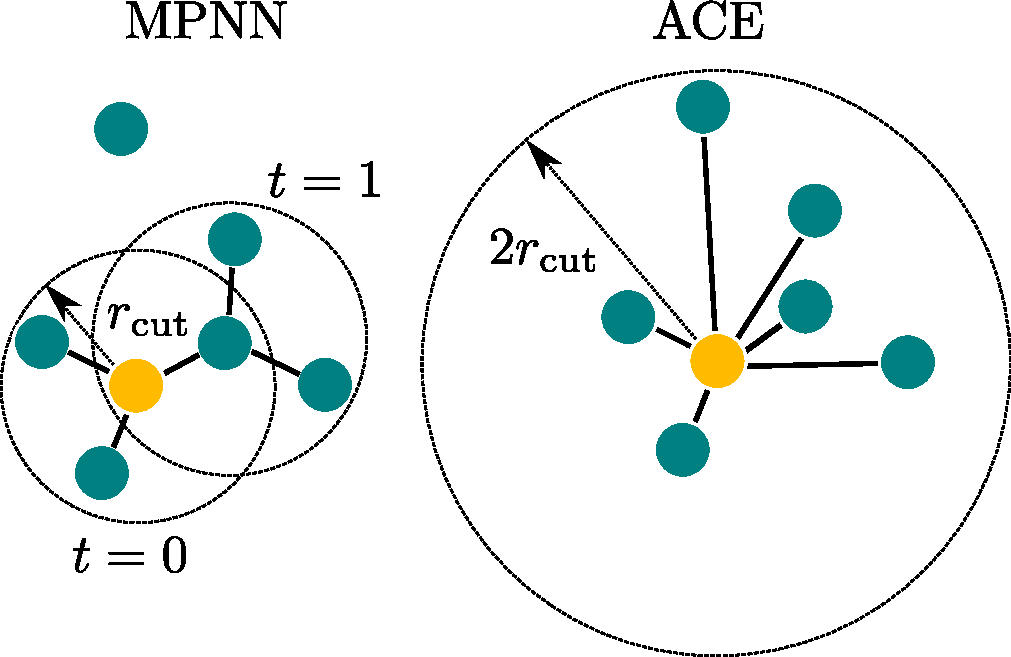
\includegraphics[scale=0.2]{figures/message_passing_schematic.pdf}
%     \caption{Caption}
%     \label{fig:my_label}
% \end{figure}

\begin{figure}[H]
    \centering
    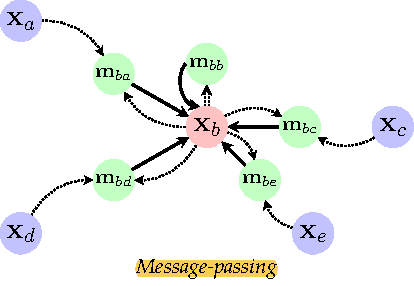
\includegraphics{figures/message-passing.pdf}
    \caption{A schematic showing a single message passing step with node $b$ aggregating messages that it receives from its neighbours $\mathcal N(b) = {a,c,d,e}$ taken from Veli\v{c}kovi\'{c} 2022 \cite{velivckovic2022message}}
    \label{fig:message-passing}
\end{figure}

GNNs for MLIPs use the message-passing paradigm over one/many layers to update node features. The feature of an atom, along with the atom type and position make up the atom state given by the tuple:

\begin{equation}
    \sigma_i^{(t)} = (\underbrace{\vec r_i, z_i}_\text{constant}, \mathbf h^{(t)}_i)
\end{equation}

This process first starts with nodes (atoms) receiving messages ($M$) from nodes it shares an edge with (i.e. its neighbours) and aggregating these messages in some permutation-invariant way ($\oplus$), as in Equation \ref{eq:msg}. Two nodes will share an edge if their distance is less than some cutoff radius, $r_c$. The aggregated message for each node is then used with the current state of the atom to update ($U$) the features, as in Equation \ref{eq:up}. Using the notation from the MACE paper \cite{batatia2022mace}. 


\begin{equation} \label{eq:msg}
    m^{(t)}_i = \bigoplus_{j \in \mathcal N(i)} m^{(t)}_{ij} = \bigoplus_{j \in \mathcal N(i)} M(\sigma^{(t)}_i, \sigma^{(t)}_j)
\end{equation}


\begin{equation} \label{eq:up}
    h^{(t+1)}_i = U(h^{(t)}_i, m^{(t)}_i)
\end{equation}

After the desired number of layers, there is graph-wide aggregation of features in some permutation invariant way and are mapped to a scalar such as energy by a readout function ($\mathcal R$), as in Equation \ref{eq:readout}.


\begin{equation} \label{eq:readout}
    E = \mathcal R (\bigoplus_i h^{(t)}_i)
\end{equation}


\subsection{Invariance and Equivariance} 


For a group element $g \in \mathcal G$ which can act on both the input space ($\{x\}$) and output space ($\{y\}$) of $f$ via the representation $D(g)$. The form of $D(g)$ is dependent on what it is acting on. If a function is not affected by the symmetry group $\mathcal G$ it is said to be $\mathcal G$-invariant. Whereas if a function transforms in the same way as the symmetry group $\mathcal G$ it is said to be $\mathcal G$-equivariant. For a mathematical definition see Equation \ref{eq:inv-equi}. 

\begin{equation} \label{eq:inv-equi}
\begin{align*} 
\mathcal G\text{-invariant:}& \quad f(x) = f(D(g) \cdot x) \\ 
\mathcal G\text{-equivariant:}& \quad D(g) \cdot f(x) = f(D(g) \cdot x) 
\end{align*}
\end{equation}

Invariant functions `throw away' the symmetries related to group $\mathcal G$ where as equivariant functions propagate these symmetries forward to the output of the function, hence the output trasnform in the same way. See Figure \ref{fig:equivariance} to see how this with how as we rotate the input (i.e the graphs) some output features i.e distances and angles are invariant whereas the vector quantity of relative position does transform in the same way. This project has layers equivariant to the Euclidean group $\mathrm O(3)$, rotations, and reflections.

\begin{figure}[H]
    \centering
    \includegraphics[scale=0.1]{figures/equivariance.png}
    \caption{As we rotate the geometric graph $90^\circ$ anti-clockwise, the invariant properties of distance $|\vec r_{ac}|, \theta$ do not change but the equivariant vector $\vec r_{ab}$ does change with the rotation}
    \label{fig:equivariance}
\end{figure}


\subsection{Tensor Operations and Abstractions}

\subsubsection{Cartesian vs. Spherical tensors} 

As discussed, the MACE architecture uses spherical tensors whereas our CMACE architecture uses Cartesian tensors. The reason that spherical tensors have been used up to this point is that they very nicely fall out from solving systems with spherical symmetry and have the same transformation properties of the $\mathrm O (3)$ group.

\textbf{Representations. } In previous equivariant models, rank-$\ell$ tensors have been represented by a linear combination of the $2\ell + 1$ spherical harmonics of the same rank, the coefficients can be put into a vector of the same size. Meanwhile Cartesian tensors of rank $\ell$ have shape $\underbrace{3\times 3 \times \cdots \times 3}_{\ell \text{times}}$

\textbf{Transformations. } Cartesian tensors also have different representations of an orthogonal transformation matrix $Q$ which we represent by $D_\ell(Q)$. For spherical tensors, these are the $(2\ell + 1)\times(2\ell+1)$ Wigner-D matrix whereas we Cartesian tensors we must transform each index individually using $\ell$ lots of the 3x3 transformation matrix $Q$ (as in Equation \ref{eq:cart-trans} for rank-3).

\begin{equation} \label{eq:cart-trans}
    T'_{ijk} = Q_{ip}Q_{jq}Q_{kr}T_{pqr}
\end{equation}

\begin{figure}
    \centering
    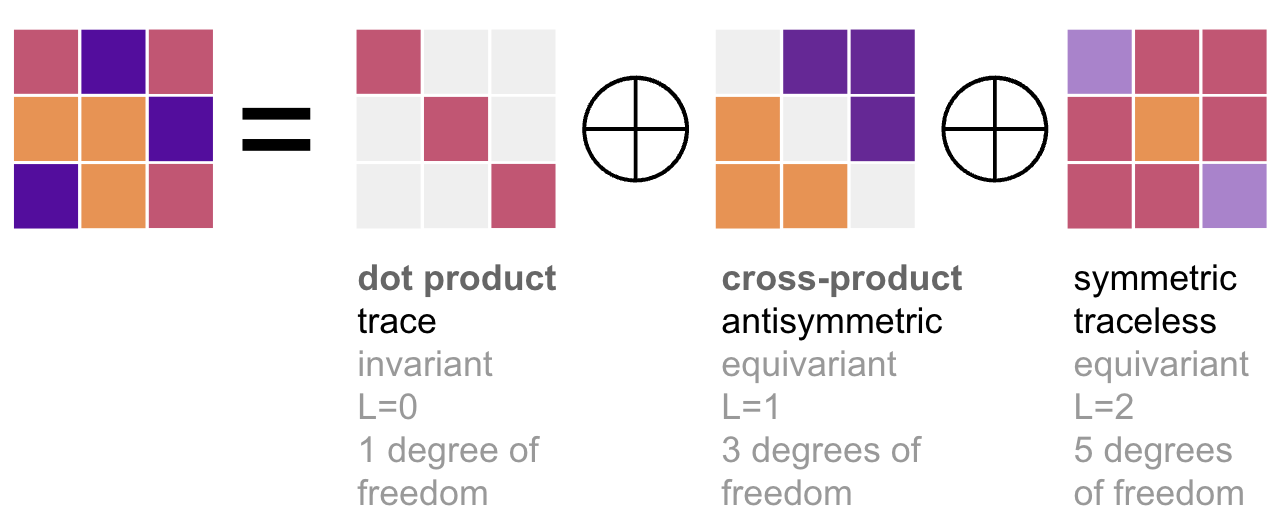
\includegraphics[width=0.76\textwidth]{figures/decomp.png}
    \caption{General matrix is a Cartesian tensor that can be decomposed into direct sum of spherical tensors with rank $0,1,2$ (Smidt 2021) \cite{Smidt2021}}
    \label{fig:decomp}
\end{figure}

\textbf{Decomposition. } Figure \ref{fig:decomp} shows that a Cartesian tensor of rank-$2$ (matrix) can be decomposed into the trace, an anti-symmetric cross product, and a symmetric traceless matrix. From this point forward, we will be using Cartesian tensors unless stated otherwise.


\subsubsection{Tensor Contractions} 
Throughout this report, the Tensor Network\footnote{\url{https://tensornetwork.org/}} notation will be used to visualise Cartesian tensors and their contractions. Much like Feynman diagrams, this notation allows for instances of combinatorial problems to be expressed with very few rules. This provides an intuitive tool in which each tensor is represented by a node and each \textit{leg} represents an index, the legs may be either free or connected to another leg, in the latter case we \textit{contract} between these two indices which in the case of Cartesian tensors amounts to setting them equal and summing (see figure \ref{fig:tensor-net}). For spherical tensors we still have the idea of contracting but this involves the Clebsch-Gordan coefficients and thus doesn't have the same intuitive visualisations - making explanations and visualisations with Cartesian tensors far simpler. 

\begin{figure}[H]
    \centering
    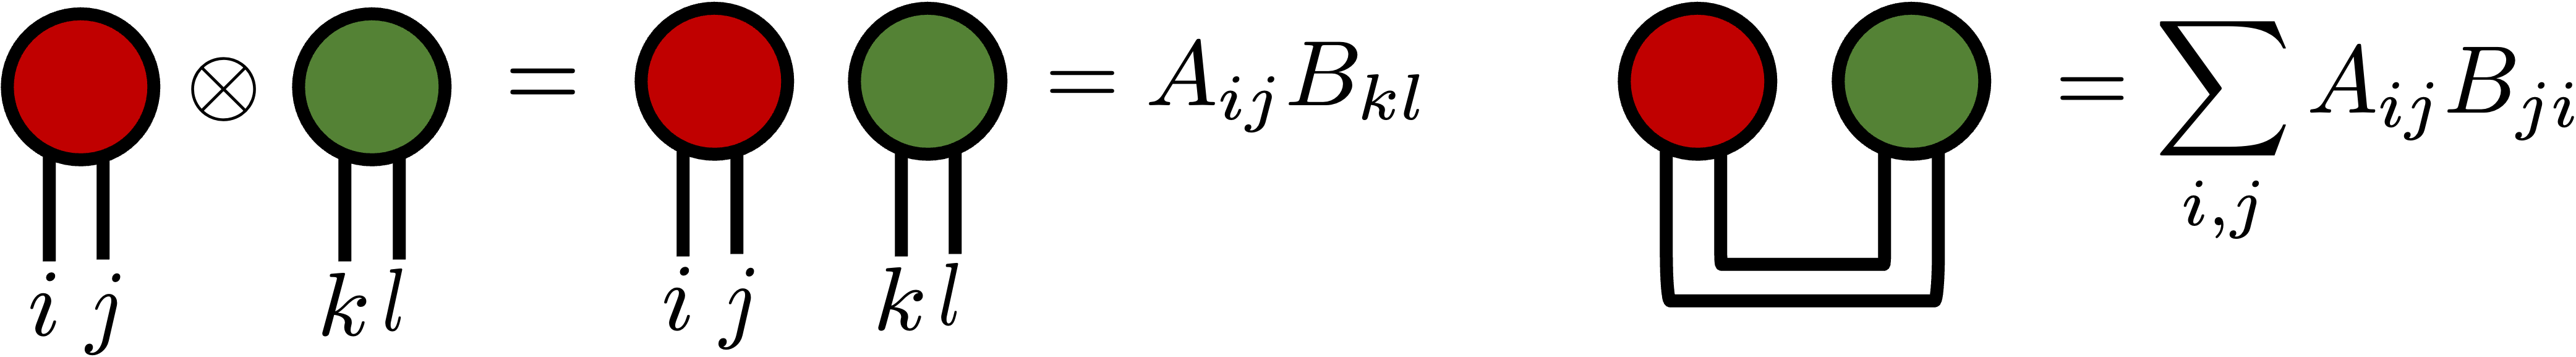
\includegraphics[scale=0.3]{figures/tensor-net.png}
    \caption{Tensor Network representation of Cartesian tensors. Here each node is a tensor and the number of legs is the number of indices. Joining two legs together is equivalent to summing over that pair of indices. Tensor products are implied when nodes are next to each other. Different node colours represents different value i.e. $A \neq B$}
    \label{fig:tensor-net}
\end{figure}

To understand the operation of our architecture we must define a \texttt{contract} operator which for a given tensor as input will produce all possible contractions of that tensor of desired output rank (the idea of the operator is not specific to Cartesian tensors). Figure \ref{fig:contraction-op} shows how to visualise this operator using tensor networks. As seen, it is only possible to get non-zero contractions when the difference between the initial and final ranks is even as contractions are done over pairs of indices. More generally, the number of different ways to do $m$ contractions to a tensor with $n$ free indices is given by equation \ref{eq:contraction-combs} (proof in Appendix \ref{sec:proof}). These contractions are symmetric and will give our layers $O(3)$ equivariance.

\begin{equation} \label{eq:contraction-combs}
    f(n,m) = \frac{n!}{(2-2m)! \cdot m! \cdot (2!)^m}
\end{equation}

\begin{figure}
    \centering
    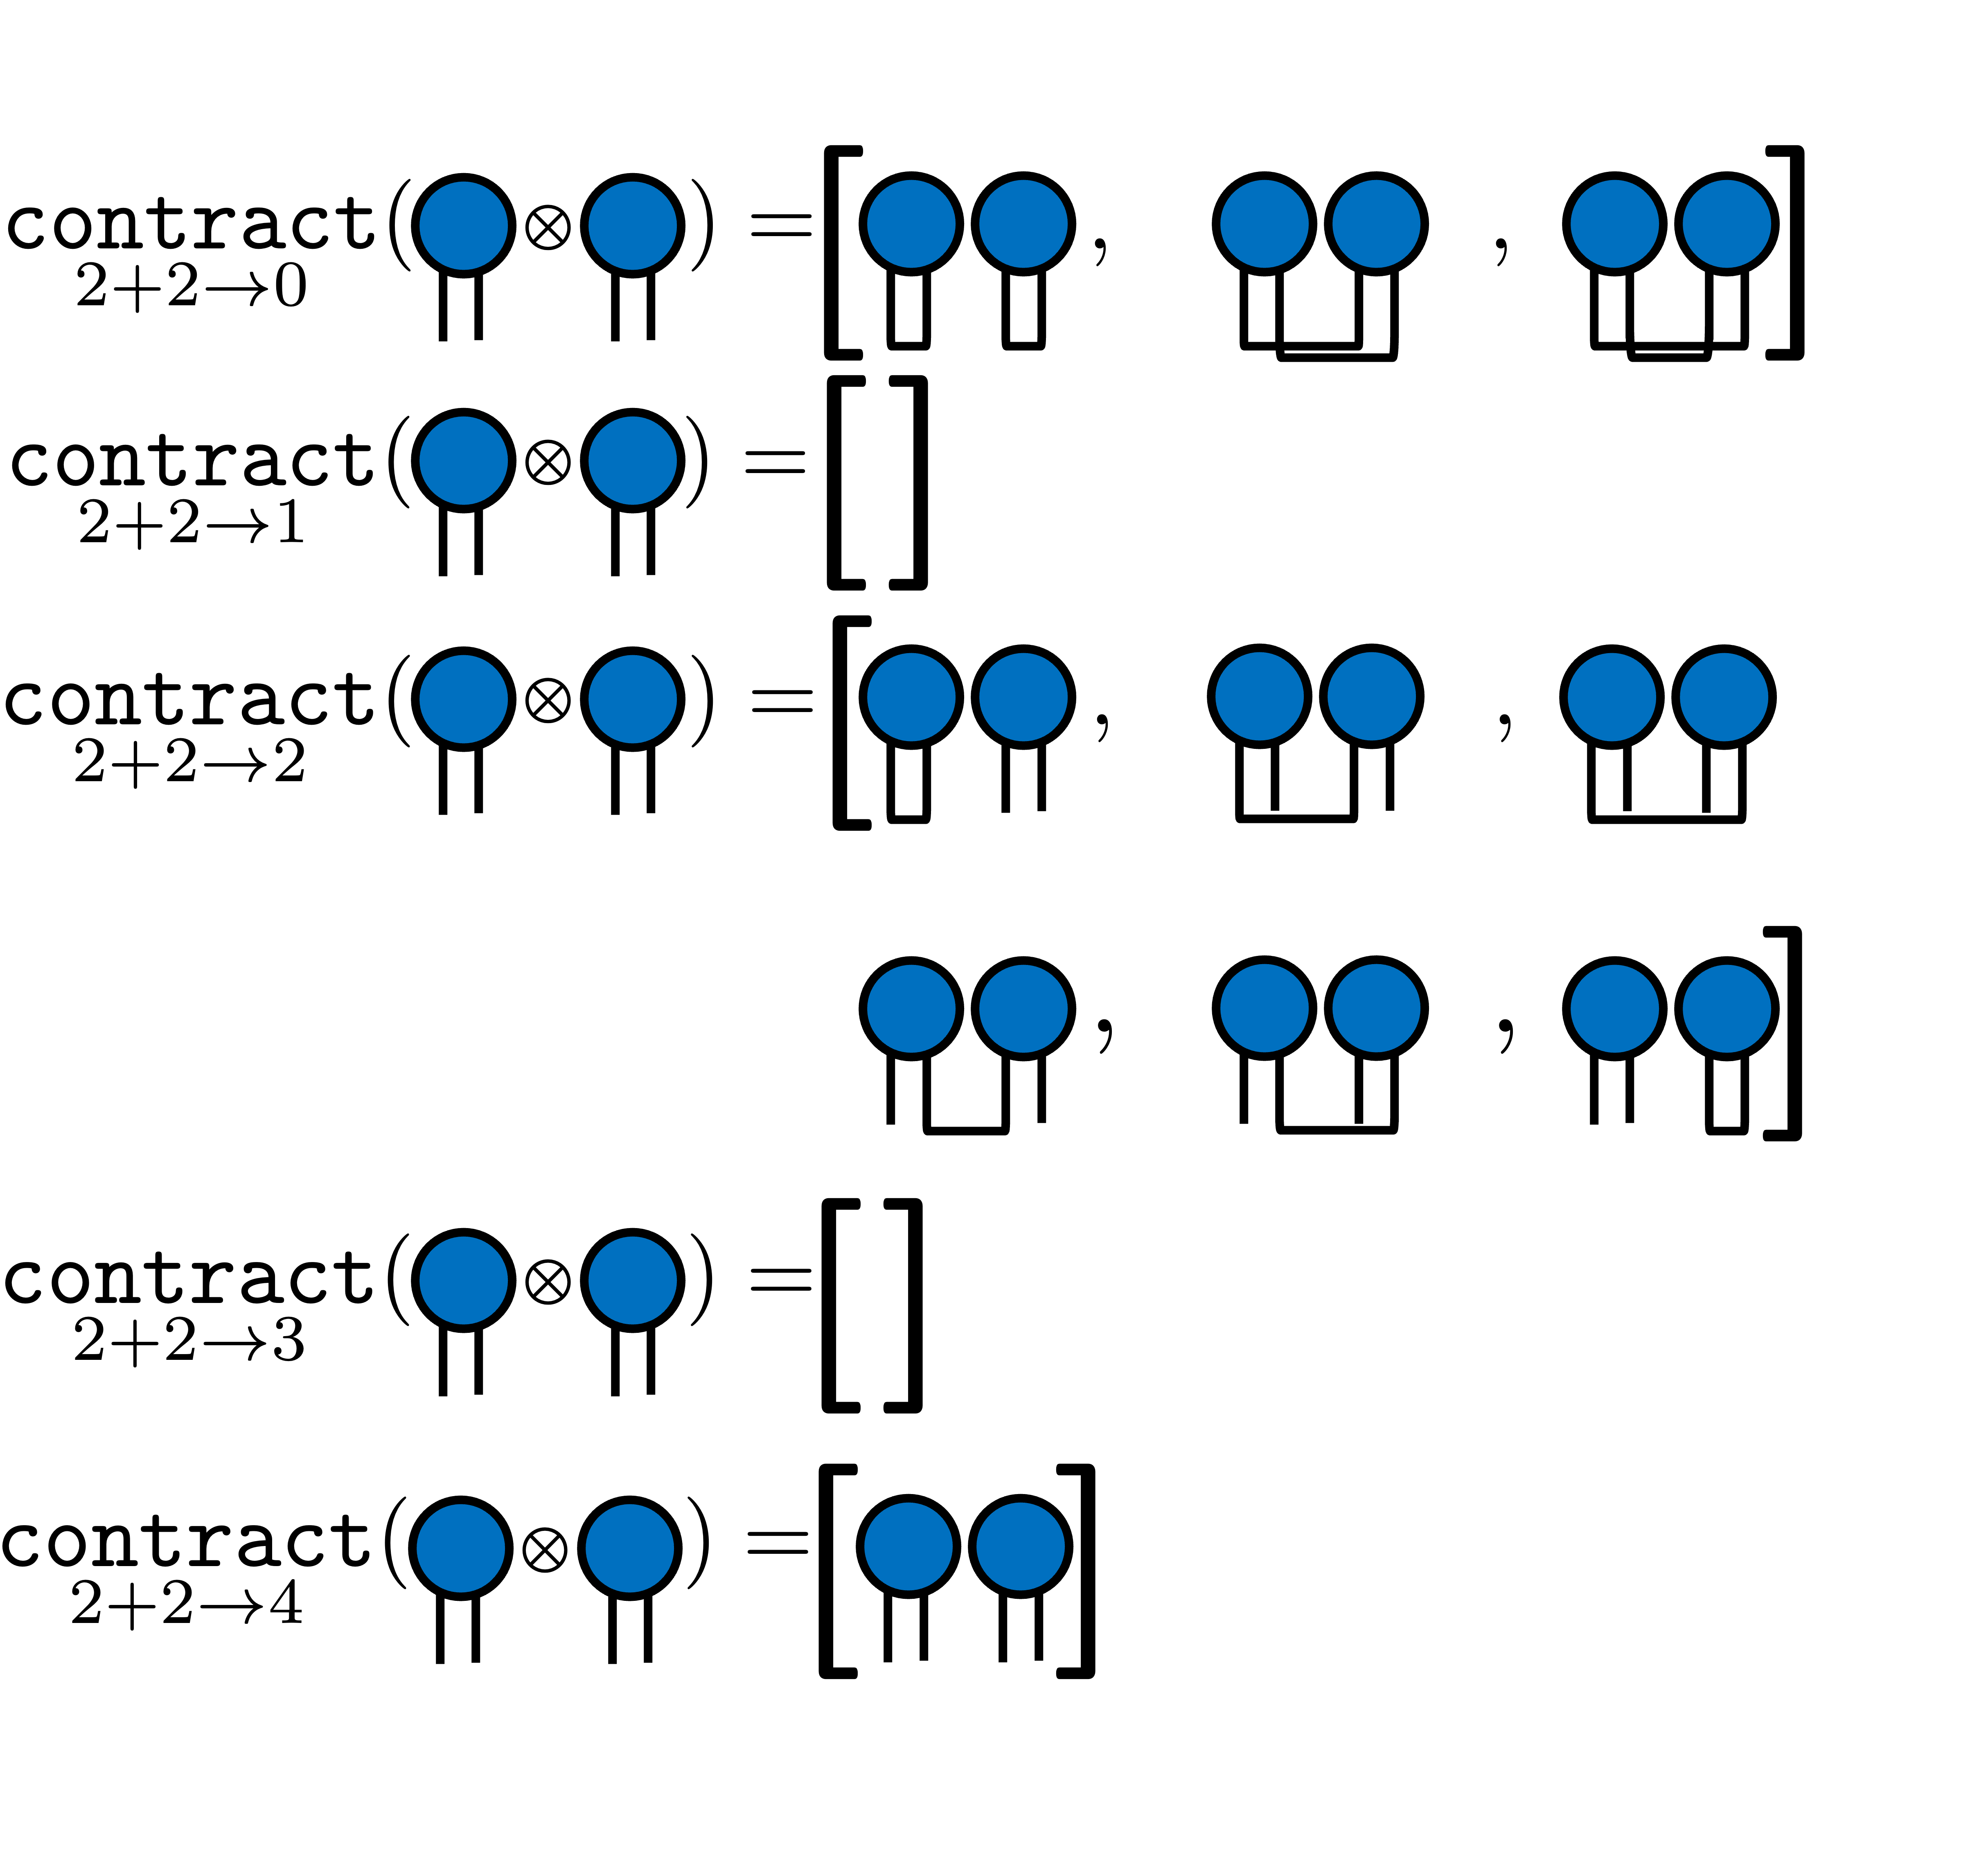
\includegraphics[width=0.7\textwidth]{figures/contraction-op.png}
    \caption{The action of the $\underset{\text{rank in} \rightarrow \text{rank out}}{\texttt{contract}}$ on a tensor of rank $2+2=4$ to ranks $0,1,2,3,4$. Output returned as a list of all possible contractions of that rank out. Contractions produce no output if rank in - rank out is not even.}
    \label{fig:contraction-op}
\end{figure}

\subsubsection{Channel mixing}

\begin{figure}[H]
    \centering
    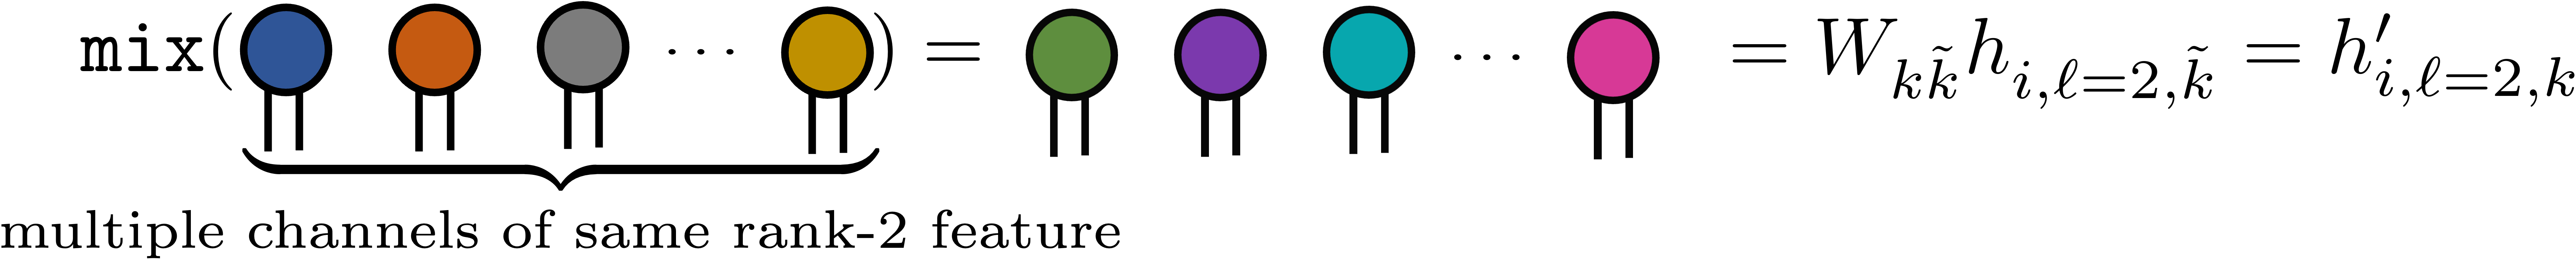
\includegraphics[scale=0.2]{figures/mixing-op.png}
    \caption{The action of the \texttt{mix} operator over the channels of a rank-2 feature. This is equivalent to linear transformation of an orthogonal weight matrix}
    \label{fig:mixing-op}
\end{figure}

In our models, as in many other machine learning models, each of the feature tensor is carried multiple times, with each copy being referred to as a `channel'. At multiple stages in the model, the channels are mixed via an orthogonal weight mate by a matrix of learned weights (unique to each instance of \texttt{mix}) over the channel index, $k$. Figure \ref{fig:mixing-op} shows the channel mixing of some rank-2 tensor features (i.e. matrices), here different colours represent different values and thus the change of colour shows the mixing. The intuition for multiple channels being useful is that different channels can focus on distinct tasks e.g. one channel might be dealing with the charge whilst another will be dealing with the bond angles. Throughout this project, the channel index is $k$ and can be ignored in all operations except for \texttt{mix}.

